\section{Versurchsaufbau}
  \label{sec:Durchführung}
  Zur Messung des Brechungsindexes $n$ von Glas und Luft wird im Versuch ein Sagnac-Inteferometer verwendet, der Versuchsaufbau ist in Abb. \ref{fig:aufbau} dargestellt.
  \begin{figure}[H]
    \centering
    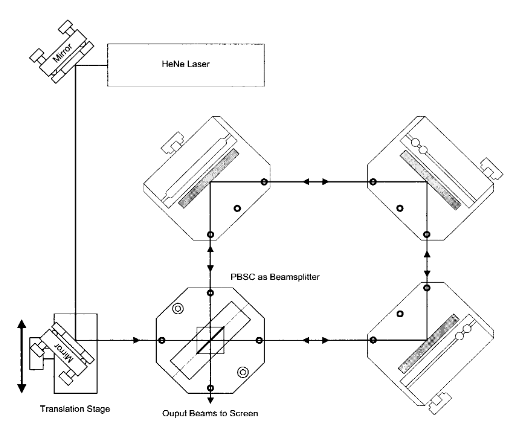
\includegraphics[width=10cm]{bilder/sagnac-interferometer,aufbau2.png}
    \caption{Versuchsaufbau zur Messung der Brechungsindizes bestehend aus dem Sagnac-Interferometer, inn diesem Versuch mit einem weiteren PBSC beim Output-Strahl und einem Polarisationsfilter vor dem ersten PBSC \cite{Anleitung}.}
    \label{fig:aufbau}
  \end{figure}
  Er besteht aus dem Sagnac-Interferometer bei dem der ausgehende rekombienierte Laserstrahl auf einen weiteren PBSC (Polarizing Beamsplitting Cube) trifft.

  Beim Sagnac-Interferometer wird durch einen HeNe-Laser ein linear polarisierter Laserstrahl der Vakuumwellenl"ange $\lambda_{vak}=\SI{632,99}{\nano \meter}$ (\cite{Anleitung}) erzeugt.
  Dieser trifft (umgelenkt durch zwei Spiegel) zun"achst auf einen Polarisationsfilter, und dann auf den ersten PBSC, einen Glasw"urfel der einen halbdurchl"assigen Spiegel enth"alt, welcher im $\SI{45}{\degree}$ Winkel zum einfallenden Strahl ausgerichtet ist.
  Dort wird der Strahl in zwei zueinander senkrecht polarisierte Strahlen (ohne Intensit"atsverlust) aufgeteilt, in dem eine Komponente den W"urfel passiert und die andere um $\SI{90}{\degree}$ abgelenkt wird.
  Die zwei Strahlen durchlaufen die Spiegel getrennt (mit einem gewissen Abstand), bis sie beim zweiten Durchgang des PBSC wieder zusammengef"uhrt/"uberlagert werden.
  Dadurch kann man die beiden Strahlen einzeln preparieren.

  %Nach einem Umlauf durch das Interferometer (alle vier Spiegel) treffen die getrennten Teilstrahlen ein weiteres mal auf den ersten PBSC, wo sie nun beim zweiten Durchlauf rekombiniert/wieder "uberlagert werden.
  Danach laufen die "uberlagerten Strahlen durch einen zweiten PBSC und die dort ausgehenden, wieder zueinander senkrecht polarisierten, Strahlen werden in je eine Photodiode geleitet, deren Spannung nun proportional zur Intensit"at des jeweiligen Lasterstrahls ist.

  Die Differenz der beiden Spannungen, oder die Spannung einer Diode kann an einem angeschlossenen Oszilloskop sichtbar gemacht werden.
  Bei "Anderung der Phasenverschiebung der beiden Strahlen (im Interferometer) "andert sich die Anzahl der Interferenzamxima/-minima um $\Delta M$, f"ur jedes neue Maximum sind die Intensit"aten der beiden Beams bei den Dioden und somit die Spannungen gleich, sodass sich ein Nulldurchgang in der Differenzspannung ergibt.
  Die Anzahl der Nulldurchg"ange der Differenzspannung kann dabei beim angeschlossenen Teach Spin Ger"at als Counts abgelesen werden.
  Beginnt die Messung mit gleichphasigen Strahlen (also keine Extrema) entspricht $\Delta M = M$.

  Weiterhin zur Verf"ugung steht ein Gaskammer, in dem mit einer Vakuumpumpe (n"aherungsweise) ein Vakuum erzeugt werden kann und eine Halterung mit zwei Glasplatten der Dicke $T=\SI{1}{\milli \meter}$ im Winkel von $\SI{10}{\degree}$ zueinander.
  Die Halterung der Glasplatten kann vertikal rotiert werden, um den Winkel $\theta$ der Glasplatten bez"uglich der Strahlen zu "andern.
  Das hei"st, bei der Knotrastmessung und der Bestimmung des Brechungsindexes $n$ von Glas durchlaufen immer beide Strahlen eine Glasplatte.



\section{Durchf"uhrung}
  Zun"achst wird das Sagnac-Interferometer nach den in der Anleitung (\cite{Anleitung}) beschriebenen Schritten 1) bis 16) eingestellt/justiert.
  Insgesamt ist das Ziel, zwei getrennte (also einzeln preparierbare) Laserstrahlen im Interferometer zu haben (die danach wieder zusammenlaufen) und m"oglichst keine Interferenzeffekte auf den Dioden zu haben, bevor die Strahlen mit Glas oder Luft prepariert werden.\\
  \\Nach der Justage wird zuerst der Kontrast $K(\phi)$ des Interferometers als Funktion des Winkels $\phi$ des Polarisationsfilters vermessen.
  Dazu wird nur die Spannung einer (beliebigen) Photodiode auf dem Oszilloskop betrachtet, jeder Strahl durchl"auft eine Glasplatte.
  Um die maximale/minimale Intensit"at bzw. Spannung zu erhalten, wird die Vorrichtung mit den beiden Glassplatten so weit gedreht, dass mehrere $2 \pi$-Phasenverschiebungen durchlaufen werden, sodass mehrere Male $I_{max}$ (Phasenverschiebung von 0) und $I_{min}$ (Phasenverschiebung von $\pi$) durchlaufen werden.
  Damit entsteht ein sinusartiger Spannungsverlauf der Diode, welcher auf dem Oszilloskop zu sehen ist. Dort wird mit den Cursorn die minimale und maximale Spannung abgelesen und notiert.
  Dies wird f"ur 10 Winkel $\phi$ des Polarisationsfilters gemacht (in 10-er Schritten von $\SI{0}{\degree}$ bis $\SI{90}{\degree}$).
  F"ur die Bestimmung der Brechungsindizes von Glas und Luft (bei Atmosph"arendruck), wird der Polarisationsfilterwinkel nun auf $\phi=\SI{45}{\degree}$ eingestellt, da hier ein maximaler Konstrast $K \approx 0,7$ vorliegt.
  Der Winkel stimmt nicht genau mit dem bestimmten Maximum aus der Ausgleichsrechnung "uberein, da die Position hier nur gesch"atzt wurde.\\
  \\Als N"achstes wird der Brechungsindex von Glas bestimmt indem die Anzahl der Interferenzmaxima/-minima $M$ als Funktion des Winkels der Glasplatten im Strahl $\theta$ bestimmt wird (siehe Abb. \ref{fig:glasplatte}).
  Daf"ur wird die Differenzspannung der Diode am Oszilloskop angezeigt.
  Nun wird die Glasplattenhalterung vier mal in $\SI{2}{\degree}$-Schritten $\SI{10}{\degree}$ weit gedreht.
  Genau wie bei der Kontrastmessung gibt es Nulldurchg"ange, wenn ein Intensit"at ein Maximum durchl"auft.
  Die Anzahl dieser Durchl"aufe wird vom Teach Spin Ger"at automatisch gez"ahlt (Counts) und muss nur noch notiert werden.\\
  \\Zum Messen des Brechungsindexes von Luft (bei Atmospherendruck) wird der optische Durchgang zun"achst auf wenige $\si{\milli \bar}$ evakuiert.
  Dann wird das Au"senventil leicht ge"offnet, sodass die Luft langsam wieder nachstr"omen kann. Dabei wird alle $\SI{100}{\milli \bar}$ bis zum Wiedererreichen des Atmospherendrucks (c.a $\SI{1}{\bar})$ die Anzahl $M$ der Interferenzmaxima/Countzahl notiert.
  Diese Messung wird drei mal durchgef"uhrt.
  Auch hier ver"andert sich der Phasenunterschied der Strahlen und somit $M$, da der Brechungsindex $n$ von Gasen druckabh"angig ist.
  F"ur die Berechnung des Brechungsindexes $n$ bei Atmospherendruck ist allerdings nur der letze Wert, also alle die Gesamtanzahl an Counts bis zum Wiederereichen des Atmospherendrucks, relevant.

%  Insgesamt wird f"unf mal $\SI{2}{\degree}$ weiter gedreht, als ein Bereich von $\SI{10}{\degree}$ abgedeckt.
%  Diese Messung wird 4 mal gleich wiederholt.
%  F"ur die Bestimmung der Brechungsindizes wird der
